\chapter{Website}

The two of the three most important prerequisites for the web platform, blockchain implementation strategy and flight delay prediction, have now been finalised. The last step is the creation of the web platform to provide a public facing insurance service for the users. The aim of the project is simplicity. Keeping that in mind, the customer should be able to buy the insurance in a way that is as transparent as possible. The internal complexity of the platform will be hidden from the user. For transparency, the user will always see the insurance payout rates before the user has to buy the insurance. The claims process, too, will be completely removed from the insurance process. The payout will be sent to the user without any user interaction required.

\section{Technologies Used}
There are multiple technologies that go towards making a full-fledged user-facing website. All the components used in making the insurance platform will be discussed in detail in this chapter. As blockchain has already been discussed in a previous chapter in detail, this chapter will only touch upon the final implementation and integration of anchoring with the website.

\subsection{Python}
Python is a dynamically scripted language that has become immensely popular in recent times due to its simplicity and huge developer support. For this project, the following two criteria were the basis on which Python was selected as the programming language of choice:
\begin{enumerate}
    \item Web frameworks
    \\Python has very popular native web-frameworks such as Django and Flask. Both have excellent documentation and developer support, essential for this project.
    \item Data science libraries
    \\ Apart from R, Python is the language with one of the most extensive support for data science libraries and a go-to choice for data science professionals. Even though the prediction algorithms were tested in R, the final implementation of the algorithm has to be in the web framework language. Hence the availability of such algorithms' native implementation in Python was an important consideration.
\end{enumerate}

\subsection{Flask}
Flask is one of the most popular frameworks in Python. Even though Django is considered to be more mature platform with higher developer support, Flask is easier to start with and had everything that was essential to create the website. 

\subsection{MySQL}
The database required for this project wasn't too complex. For this reason, the default choice, MySQL was chosen as the database.

\subsection{PyCharm IDE}
PyCharm was the Python IDE of choice for the development process as it has a free edition that provides native support for Flask framework. It also has inbuilt support for version control systems such as Github.

\subsection{Github}
For software version control, Github was chosen, being the most popular git repository service on the internet. The public account was chosen to create the repository, as it was free and the project does not require any privacy features at the moment.

\section{Website Architecture}
A custom MVC architecture was chosen for creating the website. The difference between regular and the custom implementation of MVC architecture was that no SQL queries were directly written for this website. Instead a library was used to create queries. This helps improve the security and eliminates the chances of SQL injection attacks. More details are given below in the Security section.

\subsection{User Administration}
The starting point for every user, user administration is responsible for:
\begin{enumerate}
    \item Registering a user
    \item Logging in a user
    \item Maintaining a user session
    \item Ending the user session
\end{enumerate}
A Flask library called \textit{flask\_login} was used to implement the user administration aspect of the website. A session is maintained for a particular user for 1 hour unless the user logs out before that. All the user data that is saved for a user session are encrypted by a dynamic session key by default due to the library.

\subsection{SQL model}
The SQL model defines the database model that will be used by the website for keeping user records and flight/insurance details. It contains multiple classes that correspond to unique tables in MySQL database. The first class/model defines the table structure of all the important details for the website:
\begin{itemize}
    \item First name
    \item Last name
    \item Email Address
    \item Password
    \item Flight ID
    \item Date
    \item Insurance ID
    \item Blockchain status
    \item Blockchain receipt
    \item Multiple payout amounts for different categories of delays
\end{itemize}

The second class/model defined creates a MySQL table that is used for autocomplete feature on the website. This model contains all the flight details including origin, destination, airline etc. As the insurance platform will only deal with airlines that land in Germany, the user has to be limited in his ability to enter any random flight ID. This is accomplished using the autocomplete feature of jQuery. In the Flight ID field, as soon as the user enters two characters, an autocomplete field appears which contains all the flight IDs of German flights starting with those two characters. It's a dynamic list and keeps adapting to any more characters added by the user. 

\subsection{Forms}
Forms are the flask's rendition of the HTML5 form fields. It creates HTML5 fields but adds input validation to them and makes them easier to use within the web application. The library used for flask forms is called as \textit{WTforms}. Multiple forms were created for the website like login, logout, user registration, flight details and insurance selection. 

\subsection{Views}
Views are basic functions that explain the framework what to do for each URL. For ex., when the user enters the login URL, which function to call. A Create insurance view will call a function that creates insurance and so on. The most important functions handled by views are to import and render the form, call relevant functions and add dynamic values to the forms, or adding form data to the database. 

\subsection{REST API calls}
REST API is an important component of any dynamic web application today. It is implemented using the \textit{Request} module of Python. It was used for getting flight and weather data, as well as anchoring data to blockchain. 

\subsection{Email Notifications}
The user has to be notified each time an insurance is created. If the flight has landed, the user has to be informed about the status of the insurance payout in case the flight was delayed. The notifications are currently being sent via my Gmail address using a python library called \textit{smtplib}. The user details are taken from the user table, along with the flight status and insurance payout details. This variable is passed to the library and the email is sent.

\subsection{Blockchain}
As discussed in the blockchain chapter, Tierion API is used to hash customer data and anchor it to the blockchain. This is done through a REST API call with user data sent as body in an HTTPS POST request. An ID of the request is received as the response which is stored as Insurance ID for the corresponding user in the website's database. The same insurance ID is used to renew the blockchain status and receive the blockchain receipt once the data is anchored to the blockchain.

\subsection{Insurance payout}
A script was created that runs once everyday with the help of Cron jobs. The aim of the script is to get the flight status of each flight for which the insurance was created. If a status for any flight is received, the insurance payout is decided on the basis of status. The value of the insurance payout is then sent to the user. As already mentioned, no real money is transferred to the user. Only an email with the insurance amount.

\section{Website Details}
As the backend components have been discussed, now the focus is shifted to the user interface of the website. Each webpage is discussed in detail below with the actual screenshots of the website.

\subsection{Registration Page}
The initial page for each user who wants to buy insurance through the website. As can be seen in the figure \ref{fig:reg_page}, only few basic details are required from the user to get the account ready. All the fields are input validated. The Email field should be unique for each user so that validation is also added. On clicking register, the values are again validated server side and saved in the database. The user is redirected to the login page on successful registration or shown an error if the email provided is not unique.

\begin{figure}[h]
    \centering
    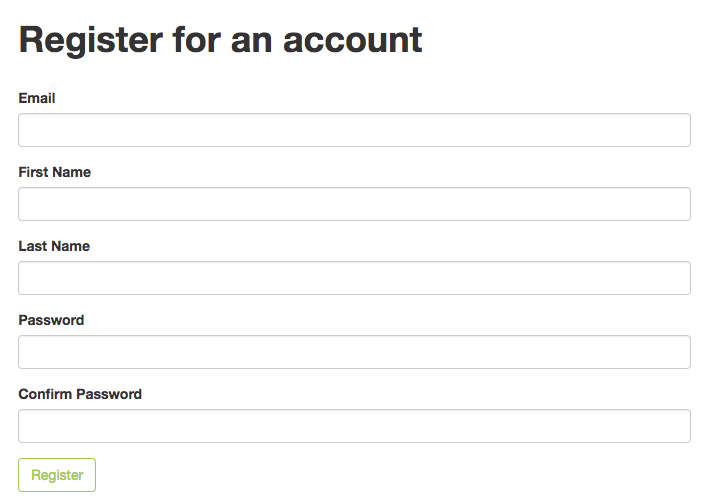
\includegraphics[width=\textwidth]{Figures/registration_page.png}
    \caption{Registration page}
    \label{fig:reg_page}
\end{figure}

\subsection{Login Page}
This is a simple login page. The user has to enter the Email ID and password and press Login. A successful login will redirect to the initial dashboard.
\begin{figure}[h]
    \centering
    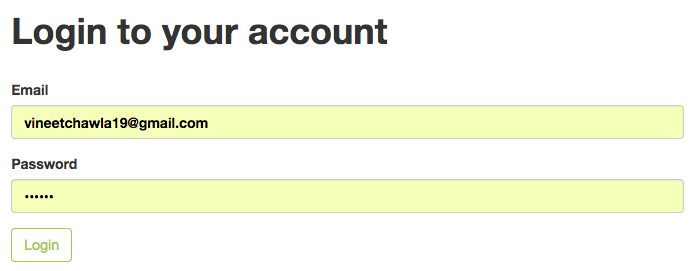
\includegraphics[width=\textwidth]{Figures/login_page.png}
    \caption{Login page}
    \label{fig:login_page}
\end{figure}

\subsection{Initial Dashboard}
The initial dashboard will be blank except for an option for adding insurance.
Once the user selects \textit{Add Insurance}, the user is redirected to Fight details webpage.
\begin{figure}[H]
    \centering
    
\includegraphics[width=\textwidth]{Figures/init_dashboard.png}
    \caption{Initial Dashboard}
    \label{fig:init_dash}
\end{figure}


\subsection{Header/Footer}
There are multiple values that are set dynamically in the header:

\begin{itemize}
    \item The rightmost field in the header is always \textit{Hi\,first\_name}.
    \item Once the user logs out, the Logout button is changed to login.
    \item The link to website's codebase in Github, \url{https://github.com/vineetchawla/InsuranceWebApp2} is also available in the header.
\end{itemize}

\begin{figure}[h]
    \centering
    
\includegraphics[width=\textwidth]{Figures/header.png}
    \caption{Header of the website}
    \label{fig:header}
\end{figure}

\subsection{Flight Details}
The flight details page is the first part of the process of booking insurance for the user. Even though there are many fields visible to the user, only two fields can be filled by user input:
\begin{itemize}
    \item Flight ID
    \\This is a drop down list where as soon as the user enters two characters, the valid flight IDs will be automatically suggested. On selecting a flight, automatically all the fields are populated with details of the flight selected. Only the suggested flight IDs will be considered valid for insurance. This auto completion is achieved using jQuery.
    \item Date
    \\ A simple date field for entering the date of the flight departure.
\end{itemize}
Once the user selects the Flight ID and date and presses \textit{Calculate Insurance rates}, the user is redirected to the screen with multiple length of flight delays with corresponding insurance payout rates.

\begin{figure}[H]
    \centering
    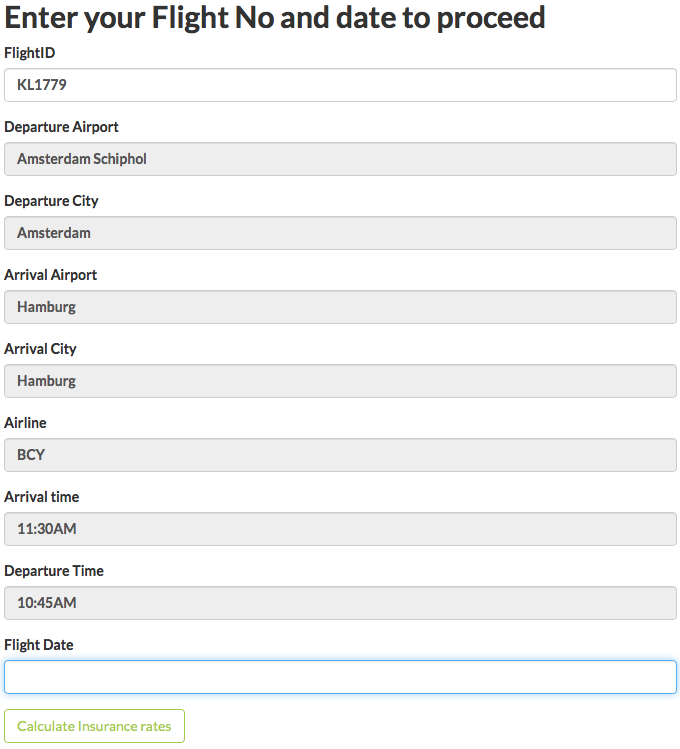
\includegraphics[width=.9\textwidth]{Figures/flight_details.png}
    \caption{Flight details}
    \label{fig:flight_details}
\end{figure}

\subsection{Insurance Rates}
Even though the previous step was a redirect, a whole lot of processing happens at the backend. The flight and weather details for the flight are requested, the received data is used to predict the flight delay using the finalised model and insurance rates are calculated based on the following criteria.

The insurance rates for each class will be calculated with the formula\\
\((60*delay\_class)/(pred\_delay\_class + 1)\), where pred\_delay\_class is the predicted delay class.

\begin{table}[H]
\centering
\begin{tabular}{l | a | b | a | b }
\hline
\rowcolor{LightCyan}
\mc{1}{}  & \mc{1}{Class 0} & \mc{1}{Class 1} & \mc{1}{Class 2} & \mc{1}{Class 3}  \\
\hline
Payout for Class 0 & 0 & 0 & 0 & 0  \\
Payout for Class 1 & 60 & 30 & 20 & 15 \\ 
Payout for Class 2 & 120 & 60 & 40 & 30\\
Payout for Class 3 & 180 & 90 & 60 & 45 \\ \hline
\end{tabular}
\caption{Insurance payout rates, with predicted classes as columns}
\label{table:payouts}
\end{table}

In the table \ref{table:payouts}, the columns are the predicted delay class. So if the algorithm predicts flight delay class 2 for a flight, the insurance payout rates would be 0, 20, 40 and 60 euros respectively. Now if the flight is delayed for 1 hour, the user receives \EUR{40}, if the flight is delayed for more than 2 hours, then \EUR{60} and so on.
\\In a bid to be completely transparent to the user, these insurance payout rates are presented before buying the insurance. If the user is satisfied with the rates he/she can move ahead and Create Insurance.

\begin{figure}[H]
    \centering
    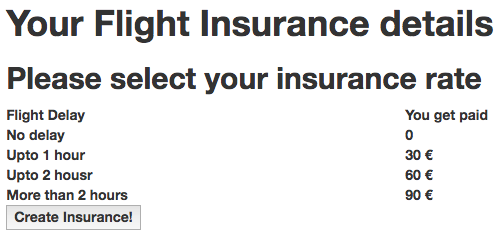
\includegraphics[width=\textwidth]{Figures/insurance_rates.png}
    \caption{Insurance rates if flight delay predicted is class 1}
    \label{fig:insurance_rates}
\end{figure}

\subsection{Dashboard}
On buying the insurance, the user is redirected to the dashboard, but this time the user will have a new table on the dashboard. This table contains all the details of the insurance the user has purchased along with the available blockchain anchoring proof, once available. Blockchain anchoring takes time due to the fundamental design of how Bitcoin works. Hence the blockchain receipt is not initially available. That's why just after creating the insurance, the dashboard will have the blockchain status as unpublished as seen in figure \ref{fig:mid_dashboard}

\begin{figure}[H]
    \centering
    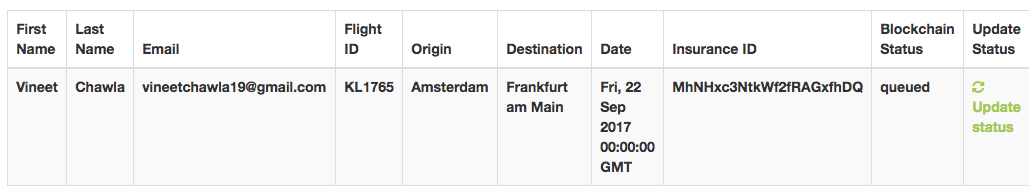
\includegraphics[width=\textwidth]{Figures/mid_dashboard.png}
    \caption{Insurance created but user details haven't been anchored to blockchain yet}
    \label{fig:mid_dashboard}
\end{figure}

The status update button is available on the dashboard, and pressing it refreshes the status. Within 10 minutes, the blockchain status will be marked as complete and blockchain receipt will be visible in the box below the table as shown in figure \ref{fig:complete_dashboard}

\begin{figure}[H]
    \centering
    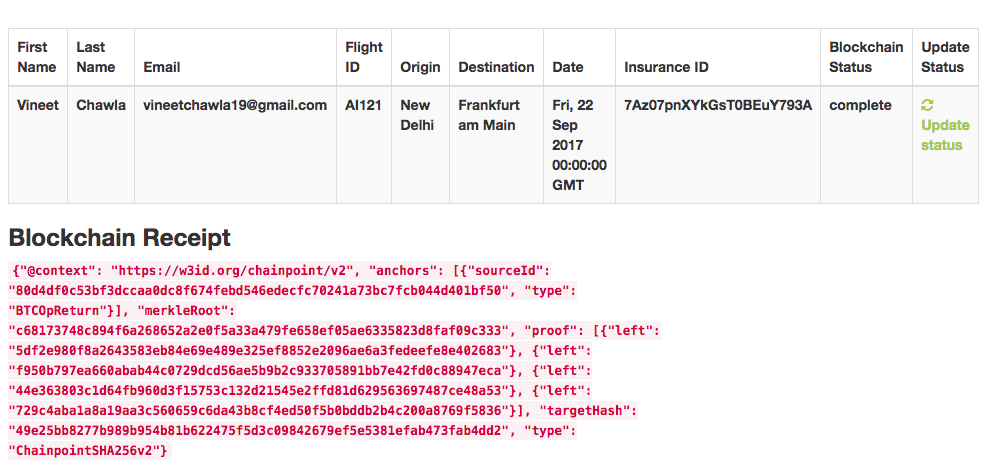
\includegraphics[width=\textwidth]{Figures/complete_dashboard.png}
    \caption{The Blockchain receipt is available and status has been updated}
    \label{fig:complete_dashboard}
\end{figure}

\section{Cloud Provider}
For hosting the website in public cloud, the consideration was for a web hosting company rather than cloud service providers like Amazon and Google. Instead of providing with empty virtual machines, pythonanywhere.com tries to automate most of the tedious work of setting up the web server, including the database creation, python libraries installation and initialisation. 
The setup ensured there is no manual oversight required for managing the web server. Once the code was downloaded from Github onto pythonanywhere's server, the website was live within minutes.


\section{Security Features}
Even though this is not a security project, the website security has been given utmost importance.
\begin{enumerate}
    \item HTTPS
    \\An HTTPS certificate from Let's Encrypt is used to encrypt connection to the website. This maintains the privacy of connection and makes sure the connection doesn't leak any confidential data.
    \item Passwords are always stored as hashes. So in case of an attack, the attacker will never get to know the real passwords.
    \item There is not a single SQL query in the entire application. Creating SQL queries is handled by the library \textit{SQLAlchemy} instead. The type of query with the parameters is sent to the library and the library does the rest. As a result, chances of SQL injection attacks are completely eliminated.
    \item Every user input is validated at the client side as well as server side.
    \item The user's session variables are encrypted to prevent data leakage.
\end{enumerate}

